\appendix
\titleformat{\chapter}[block]{\vspace*{-2.5cm}\normalfont\Large\bfseries}{Appendix \thechapter \;\textendash\;}{0ex}{\vspace{-4cm}}[\vspace{4.5cm}]
\titlespacing{\chapter}{0cm}{0cm}{0cm}

\chapter{Exploring the Energy Function}
\label{chap:memo-on-the-energy}
In an attempt to find an explicit expression of the energy function $E(\alpha, \beta, R, d)$, we plotted and fitted the energy function in $\alpha$ and $R$ so that it can be visualised with $d = 1$ and $\beta = 0.4$ held constant.

The fit of $E(\alpha, R)$ depicted in \Cref{fig:multivariate-energy-3d} is done by minimising the square error between energy values returned by the solver and the following function:
\begin{align*}
  E(\alpha, R; \vec{x}) = & x_{1} + \alpha \cdot x_{2} + \alpha^2 \cdot x_{3} + \alpha^3 \cdot x_{4} + R^\alpha \cdot x_{5} + R^\beta \cdot x_{6} \\
                          & + R \cdot x_{7} + R^2 \cdot x_{8} + R^3 \cdot x_{9} + R^4 \cdot x_{10} + \log(\alpha) \cdot x_{11}\,.
\end{align*}

% [-3.2290656926194745, 4.191742247704756, -0.9901655688595846, 0.1054275395353191, -0.1508895211749961, -1.9114728748086454, 0.132376743248443, 0.6617933016251011, -0.12573696508776597, -0.02991876184227984, -3.1864697903599177]
The resulting best-fit parameter combination is
$$\vec{x}_{\rm min} = (
  -3.22,
  4.19,
  -0.99,
  0.11,
  -0.15,
  -1.91,
  0.13,
  0.66,
  -0.13,
  -0.03,
  -3.18
  )^T\,.$$
as obtained through Optim.jl's \gls{lbfgs} minimisation routine \parencite{2023-optim-jl} with \gls{ad} for the gradient.

\begin{figure}[H]
  \centering
  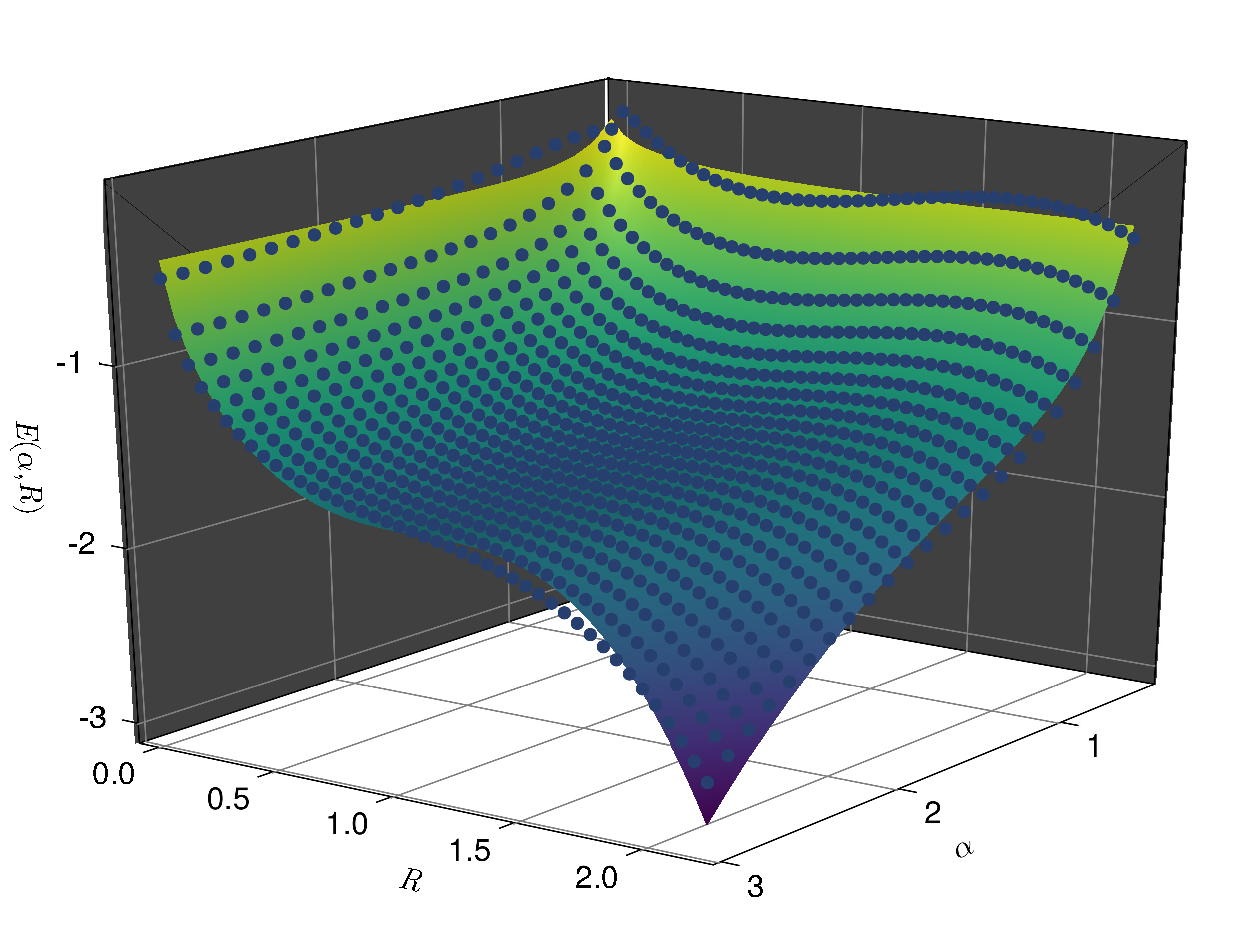
\includegraphics[width=0.7\linewidth]{results/attrep/multivariate-energy-3d.pdf}
  \caption[Surface plot of the total potential energy $E(\alpha, R)$]{Surface plot of the total potential energy $E(\alpha, R)$, the blue scatter points represent the fit $E(\alpha, R; \vec{x}_{\rm min})$.}
  \label{fig:multivariate-energy-3d}
\end{figure}

The conclusion seems to be that the behaviour is highly non-polynomial, even when using powers $R^\alpha$ and $R^\beta$, etc. instead of only monomials.
One could expect this given the analytical energy expressions in \Cref{sec:analytical-solutions} and \cite{2017-explicit-solutions}.
Even adding in some of the terms ($B(\cdot, \cdot) \cdot \cos(\cdot)$, etc.) from the analytical expressions did not help.
We also tried higher orders in $\alpha$, $R$, more log terms, cross-terms, and we even experimented with the beta function.

\chapter{Various Plots}
\label{appendix:various-plots}
\Cref{fig:bump-solutions} depicts a ``bump'' solution resulting from an attractive-repulsive interaction kernel.
The pseudo energy dependence on position $\vec{x}$ (and due to radial symmetry, on $r$) for different support radii $R$ is given in \Cref{fig:spatial-energy-dependence}.
Instead of taking energy as the average $\bar{I}_{m,n}^{(\alpha,\beta)}$, one can use ${I}_{m,n}^{(\alpha,\beta)}(\vec{x})$.
\Cref{fig:varying-parameters} illustrates the effects of various parameters in the attractive-repulsive case.

\begin{figure}[H]
  \centering
  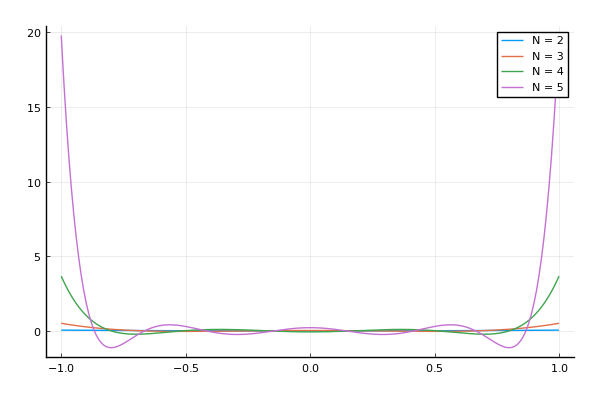
\includegraphics[width=0.8\linewidth]{results/bump/solution-increasing-order}
  \caption[Bump parameter solutions]{Solutions with bump parameters.}
  \label{fig:bump-solutions}
\end{figure}

\begin{figure}[H]
  \centering
  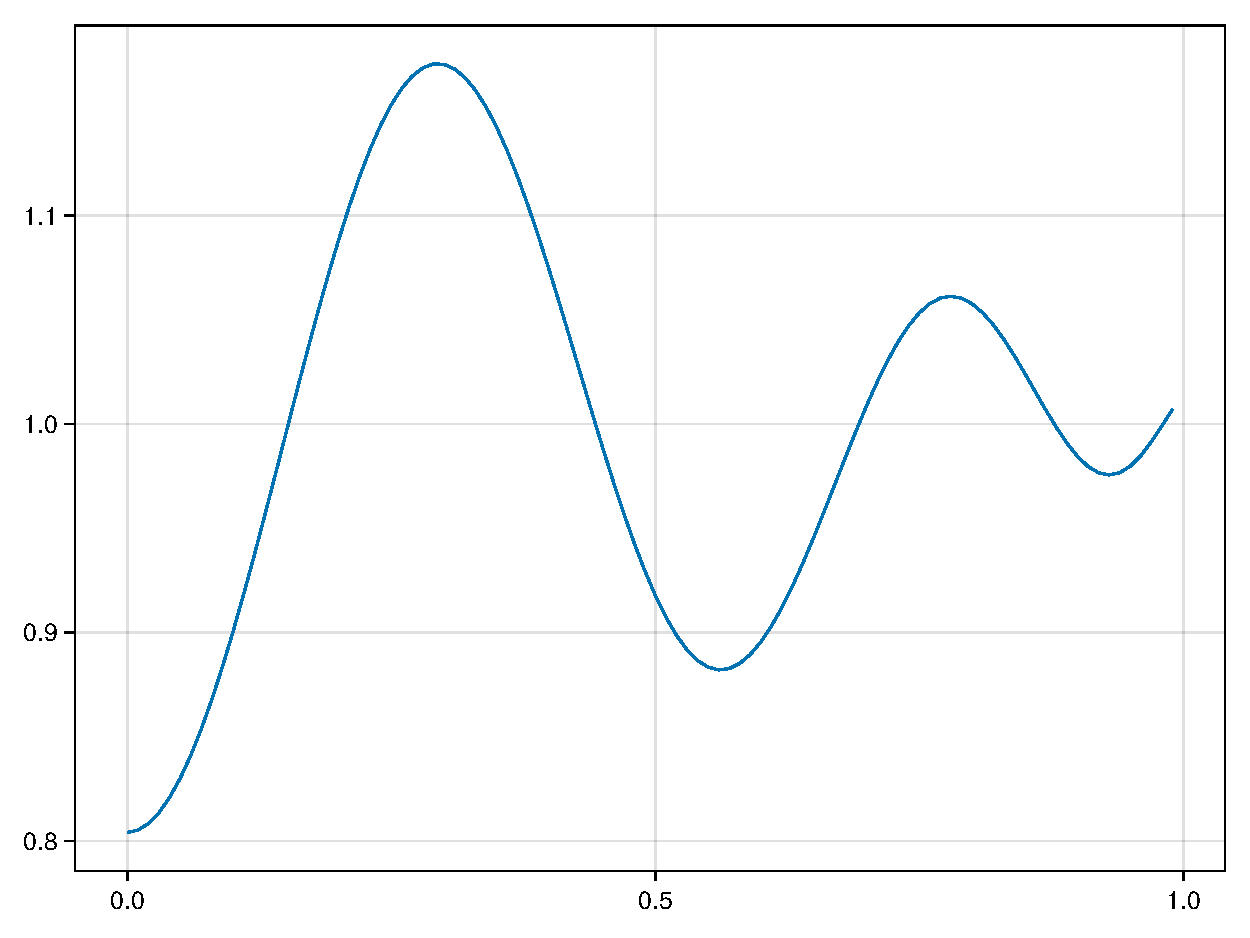
\includegraphics[width=0.8\linewidth]{results/attrep/energy-dependence-on-r.pdf}
  \caption[Spatial energy dependence on $r$]{Plot of the spatial energy dependence on $r$, for different values of the domain support radius $R$. As one can see, $\tilde{E}(\vec{x}) = \sum_{k=0}^{N-1} \rho_k {I}_{m,n}^{(\alpha,\beta)}(\vec{x})$ is roughly constant and this figure is only present as visual proof to increase our confidence in the construction of the spectral method.}
  \label{fig:spatial-energy-dependence}
\end{figure}
\pagebreak

An example of collective motion arising from the mixed potential is given in \Cref{fig:mixed-2d-quiver}.

\begin{figure}[H]
  \centering
  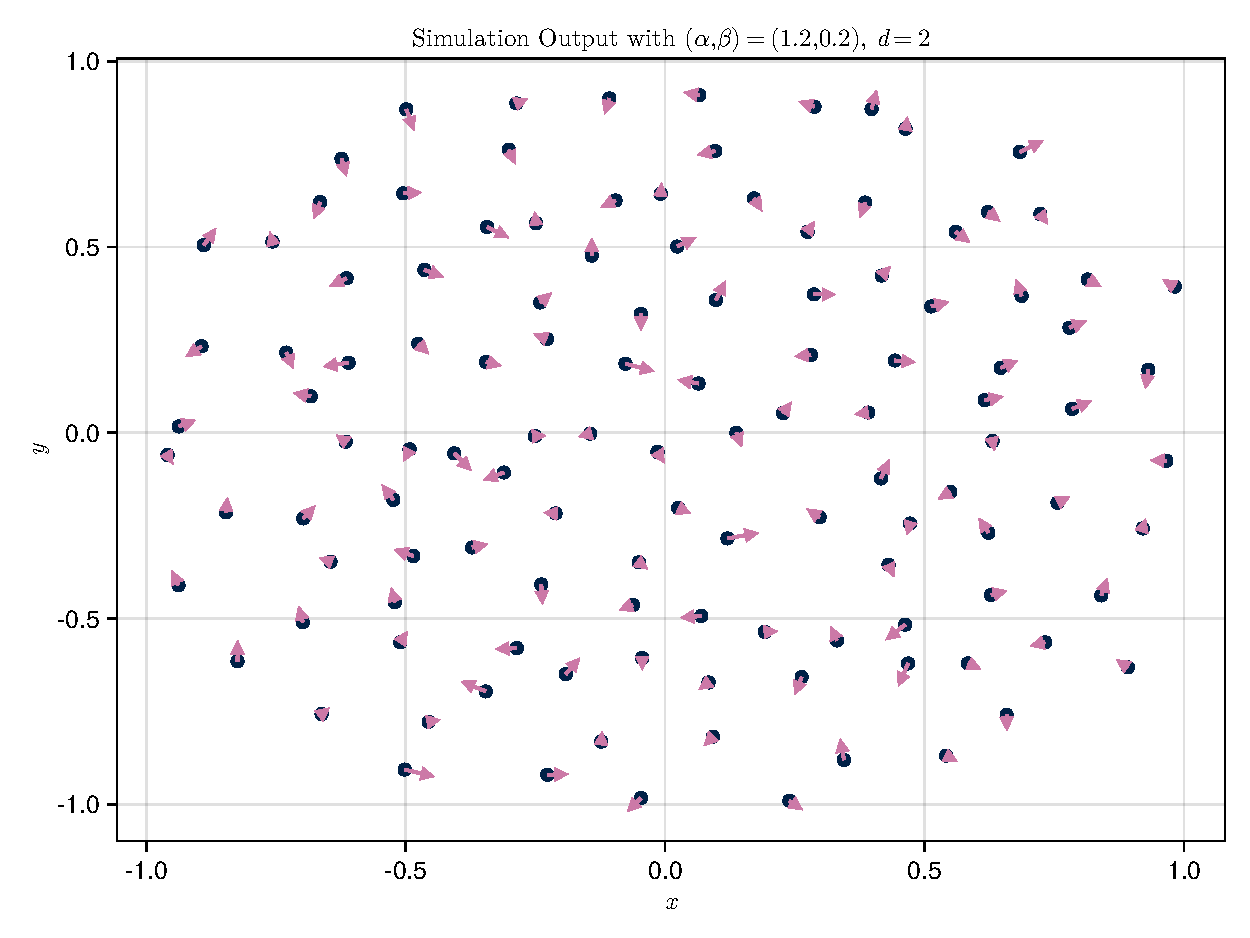
\includegraphics[width=0.8\linewidth]{results/mixed-2d/simulation-quiver.pdf}
  \caption[2D quiver plot for the mixed potential]{$N_p = 200$ particles interacting through the mixed potential $K_{(C, l, \bar{a})}(r) := \frac{r^{\bar{a}}}{\bar{a}} + C e^{-r/l}$ (cf. \Cref{eq:mixed-potential}) in \Cref{chap:particle-interaction-theory}.}
  \label{fig:mixed-2d-quiver}
\end{figure}

\pagebreak
\begin{figure}[H]
  \centering
  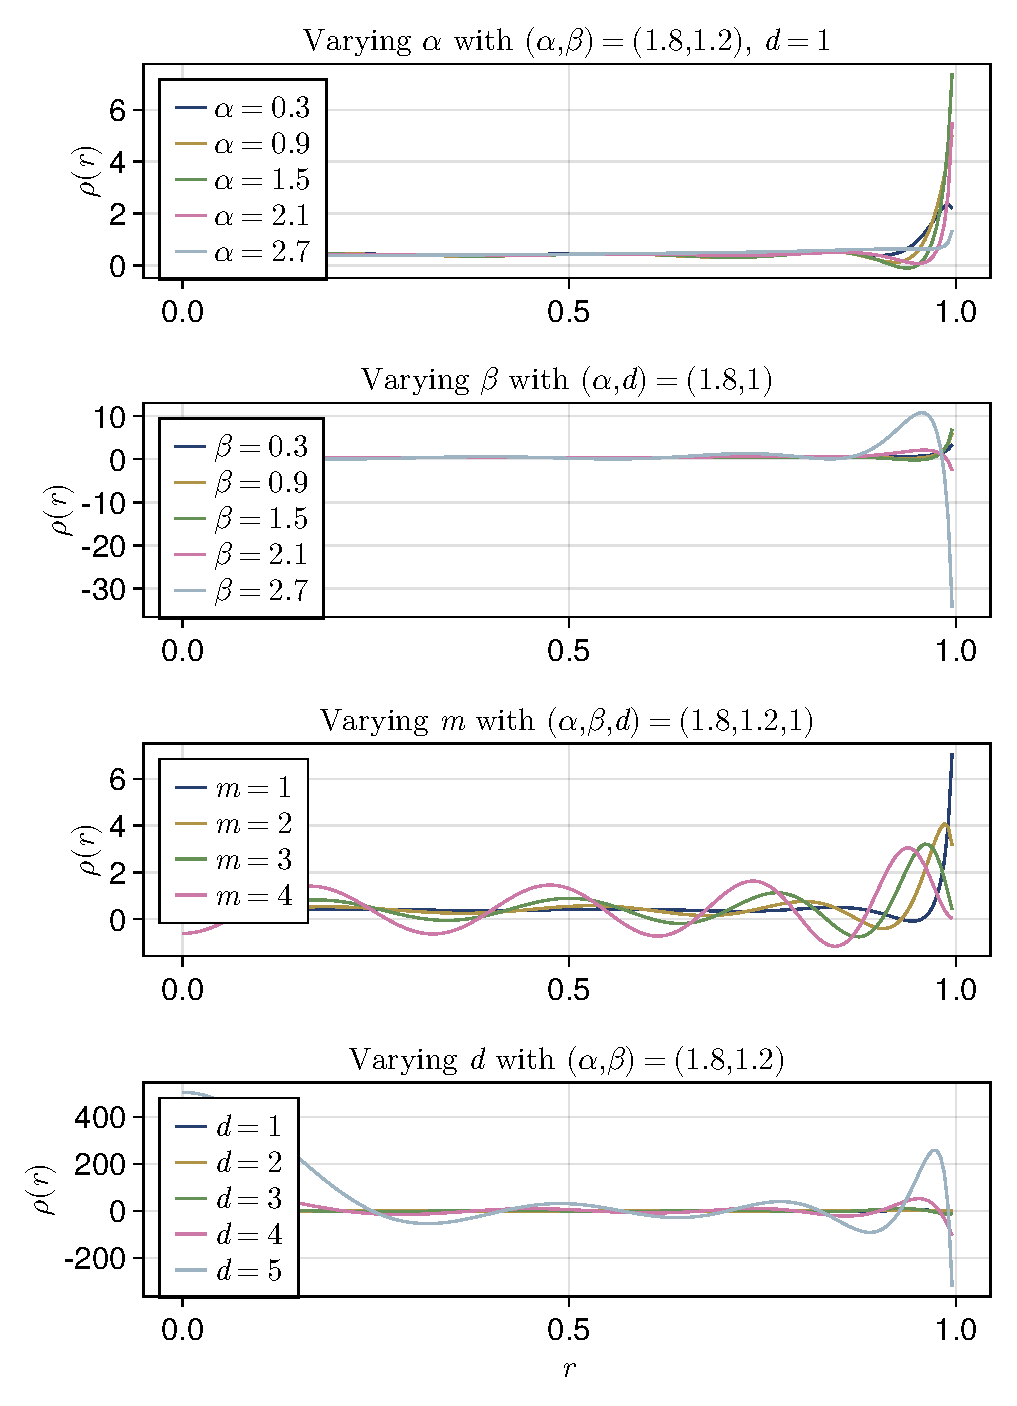
\includegraphics[width=0.9\linewidth]{results/attrep/varying-parameters.pdf}
  \caption[Varying parameters in the solver]{
    Varying different parameters in the solver to demonstrate their effect.
    See also, \Cref{fig:varying-R-solutions}.
  }
  \label{fig:varying-parameters}
\end{figure}
\pagebreak

\chapter{Code Snippets}
\label{appendix:code-snippets}

\section{Leapfrog Integration}
\begin{minted}{cpp}
void ParticleBox::simulate(size_t timesteps) {
  double afterAccelerations[PARTICLES][DIMENSION];
  f(afterAccelerations);
  for (size_t t = 0; t < timesteps; t++) {
    ParticleVectors beforeAccelerations = afterAccelerations;
    memcpy(beforeAccelerations, afterAccelerations, PARTICLES * DIMENSION * sizeof(double));
    for (size_t i = 0; i < PARTICLES; i++) {
      for (size_t d = 0; d < DIMENSION; d++)
        positions[i][d] += p.tau * velocities[i][d] + square(p.tau) / 2 * beforeAccelerations[i][d];
    }

    f(afterAccelerations);
    for (size_t i = 0; i < PARTICLES; i++) {
      for (size_t d = 0; d < DIMENSION; d++) {
        velocities[i][d] += (p.tau / 2 * (beforeAccelerations[i][d] + afterAccelerations[i][d])) / p.boxScaling;
      }
    }
    reflectParticles();
  }
}
\end{minted}

\pagebreak
\section{Operator Construction without Recurrence}
\begin{minted}{julia}
OpMem = LRUCache.LRU{Tuple{Int64, Float64,SolutionEnvironment}, Matrix{BigFloat}}(maxsize=20)
"""Creates a power law operator given alpha and beta. Caches it."""
function constructOperator(N::Int64, beta::Float64, env::SolutionEnvironment)::Matrix{BigFloat}
  get!(OpMem, (N, beta, env)) do
    Mat = zeros(BigFloat, N, N)
    r_axis = axes(env.P, 1)
    for n in 0:N-1
      Function = Utils.theorem216.(r_axis; n=n, beta=beta, p=env.p)
      ExpansionCoeffs = env.P[:, 1:N] \ Function  # expands the function in the P basis
      Mat[:, n+1] .= ExpansionCoeffs
    end
    Utils.zeroOutTinyValues!(Mat)
    Mat
  end
end
\end{minted}
